\documentclass[11pt, oneside]{article}   	% use "amsart" instead of "article" for AMSLaTeX format
\usepackage{geometry}                		% See geometry.pdf to learn the layout options. There are lots.
\geometry{letterpaper}                   		% ... or a4paper or a5paper or ... 
%\geometry{landscape}                		% Activate for for rotated page geometry
%\usepackage[parfill]{parskip}    		% Activate to begin paragraphs with an empty line rather than an indent
\usepackage{graphicx}				% Use pdf, png, jpg, or eps� with pdflatex; use eps in DVI mode
								% TeX will automatically convert eps --> pdf in pdflatex		
\usepackage{amssymb}
\usepackage{amsmath}
\usepackage{parskip}
\usepackage{color}

\title{Stokes Theorem and the divergence}
%\author{The Author}
%\section{}
% \subsection*{R code}
\date{}							% Activate to display a given date or no date

\graphicspath{{/Users/telliott_admin/Dropbox/Tex/png/}}

% \begin{center} 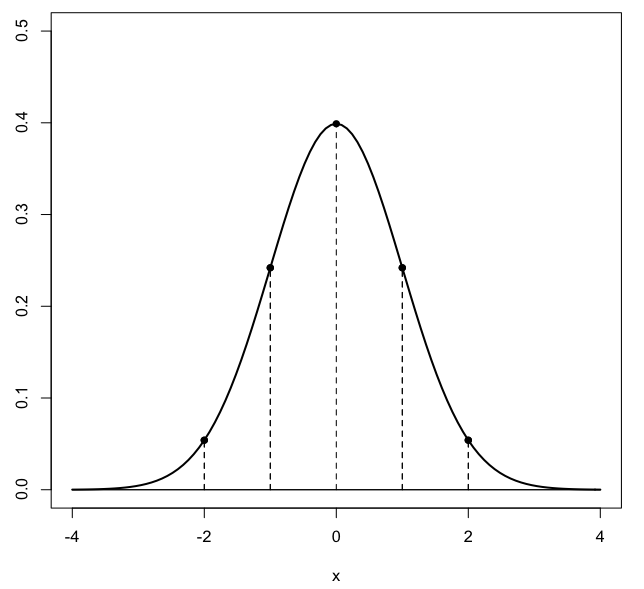
\includegraphics [scale=0.4] {gauss3.png} \end{center}
% \begin{bmatrix} a  &  b \\ c  &  d \end{bmatrix}
% \bigg |_

\begin{document}
\maketitle
\large
%\noindent
\subsection*{Stokes}

\[ \oint_C \mathbf{F} \cdot d \mathbf{r} = \iint_S ( \nabla \times \mathbf{F}) \cdot \hat{\mathbf{n}} \ dS \]
Stokes' theorem applies to a curve in space (it does not have to lie in a plane).  The theorem says that the work going around the curve is equal to the integral over \emph{any surface} with that curve as its boundary, of the component of the curl of $\mathbf{F}$ normal to the surface. 

An alternative form (using the fact that $\mathbf{dr} = \langle dx,dy,dz \rangle$, and computing the curl $\nabla \times \mathbf{F}$) is

\[ \int_C P \ dx + Q \ dy + R \ dz = \iint_R   \ <R_y-Q_z,P_z-R_x,Q_x-P_y> \  \cdot  \hat{\mathbf{n}} \ dS \]

When Stokes' theorem is applied to a region in the $xy$-plane, $\hat{\mathbf{n}} = \hat{\mathbf{k}}$, so only the third term of the curl is non-zero, and $dS = dA$.  On the left-hand side $dz=0$, so this just reduces to

\[  \int_C P \ dx + Q \ dy  = \iint_R \ (Q_x-P_y) \ dA \]

which is Green's theorem for work.

\subsection*{Divergence in space}

The last theorem is called the divergence theorem, or Gauss's theorem (and there are other names).

\[ \iint_S \mathbf{F} \cdot \mathbf{n} \ dS  = \iiint_V \ \nabla \cdot \mathbf{F} \ dV \]
\[ =  \iiint_V \ (P_x + Q_y + R_z )\ dV \]

As a simple example, consider the unit sphere and a radial field $\mathbf{F} = \langle x,y,z \rangle$.  We can certainly do the surface integral, but notice that $\nabla \cdot \mathbf{F} = 3$.  Using the theorem, the result (the flux out of the sphere) is simply $3$ times the volume of the unit sphere, or $4 \pi$.

\subsection*{Other coordinates}

Above, in $R3$, the divergence was given as

\[ \iiint_V \ \nabla \cdot \mathbf{F} \ dV \]

The "del" operator is
\[ \nabla = \ < \frac{\partial}{\partial x},\frac{\partial}{\partial y},\frac{\partial}{\partial z} > \]
The divergence of $\mathbf{F}$ is
\[ \nabla \cdot \mathbf{F} \]
if $\mathbf{F} = \ <P,Q,R>$
\[ \nabla \cdot \mathbf{F} = P_x + Q_y + R_z \]
The divergence of a vector field is a scalar quantity.

In cylindrical and spherical coordinates, the divergence is more complicated.  Although the expression above is often given as the \emph{definition} of divergence, Schey makes a big deal out of saying that he prefers this definition

\[ div \ \mathbf{F} = \lim_{\Delta V \rightarrow 0} \frac{1}{\Delta V} \iint_S \ \mathbf{F} \cdot \hat{\mathbf{n}} \ dS \]

As further illustration, the divergence has a more complicated form in cylindrical and spherical coordinates.  In the former it is 

\[ div \ \mathbf{\mathbf{F}} = \frac{1}{r} \frac{\partial}{\partial r} (rF_r) +  \frac{1}{r} \frac{\partial}{\partial \theta} (F_{\theta}) + \frac{\partial}{\partial z} (F_z) \]

where $F_{z}$ is not a partial derivative but just the component of $\mathbf{F}$ in the z-direction, and so on.

Similarly, in spherical coordinates the divergence is

\[ div \  \mathbf{\mathbf{F}} = \frac{1}{r^2} \frac{\partial}{\partial r} (r^2F_r) +  \frac{1}{r \ \sin \phi} \frac{\partial}{\partial \phi} (\sin \phi F_{\phi}) + \frac{1}{r \ \sin \phi} \frac{\partial}{\partial \theta} (F_{\theta}) \]

\subsection*{example}

Here is an example to explore divergence in cylindrical coordinates.  Suppose we have a cylinder oriented along the $z$-axis with its length equal to $1$ and its radius $r=2$.  

Further, we have a field with some divergence, like $\mathbf{F} = \langle x,y,0 \rangle$.

This field is written in $x,y,z$ coordinates, when we switch to cylindrical coordinates (of course) $x = r \cos \theta$ and $y = r \sin \theta$.

We want to check the divergence theorem 
\[ \iint_S \mathbf{F} \cdot \mathbf{n} \ dS  = \iiint_V \ \nabla \cdot \mathbf{F} \ dV \]

(The integral above is an integral over a closed surface, in this case, the cylinder with top and bottom included). 

When we rewrite $\mathbf{F}$ in cylindrical coordinates, we will have 
\[ \mathbf{F} = \langle r, \theta, z \rangle \]
The given field is independent of $\theta$ and $z$ and and since
\[ r = \sqrt{x^2 + y^2} \]
\[ \mathbf{F} = \langle r, 0, 0 \rangle \]

Using the definition of divergence from above, we have
\[ div \ \mathbf{\mathbf{F}} = \frac{1}{r} \frac{\partial}{\partial r} (rF_r) +  \frac{1}{r} \frac{\partial}{\partial \theta} (F_{\theta}) + \frac{\partial}{\partial z} (F_z) \]
since $\mathbf{F}$ has no $z$ or $\theta$ component and the $r$ component is $F_r =r$ (this is \emph{not} a derivative), we have  
\[ div \ \mathbf{\mathbf{F}} = \frac{1}{r} \frac{\partial}{\partial r} (r^2) = 2 \]
So the triple integral uses the cylindrical volume element and is just
\[ \int_0^{2 \pi} \ \int_0^{1} \ \int_0^2 \ 2 \ r \ dr \ dz \ d \theta  \]
\[ = \int_0^{2 \pi} \ \int_0^{1} \ [ \ r^2 \ \bigg |_0^2 \ ] \ dz \ d \theta = 8 \pi \]
Notice that the value of the integral scales linearly with $z$ and like $r^2$.
Now for the surface integral.  In standard form, the cylinder has 
\[ \hat{\mathbf{n}} \ dS = \langle x, y, 0 \rangle \ d \theta \ dz \]
\[  \iint_S \mathbf{F} \cdot \mathbf{n} \ dS  = \langle x, y, 0 \rangle \cdot \langle x, y, 0 \rangle \ d \theta \ dz \]
\[  \iint_S x^2 + y^2  \ d \theta \ dz \]
\[  \int_0^1 \ \int_0^{2 \pi} \ r^2  \ d \theta \ dz = 2 \pi r^2 = 8 \pi \]
I almost forgot the top and bottom of the cylinder.  However the flux $\mathbf{F} \cdot \hat{\mathbf{n}} = 0$ everywhere on these two surfaces, so the total is still just $8 \pi$.

\end{document}  